\documentclass[10pt,a4paper]{article}
\usepackage[utf8]{inputenc}
\usepackage[italian]{babel}
\usepackage{amsmath}
\usepackage{amsfonts}
\usepackage{amssymb}
\usepackage{graphicx}
\author{Danilo "Bestbug" Giordani}
\title{Appunti crittografia I}


\begin{document}
\maketitle
\section{Prefazione}
La crittografia è lo studio e progettazione di algoritmi , assieme alla crittoanalisi (studio della forza di un crifrario) forma la crittologia. La crittografia fa parte della teoria dei codici: tecniche utilizzate per trasmettere e memorizzare le informazioni su un canale rumoroso. Nello specifico la crittografia dice come rendere sicuro questo canale. Nelle analisi che andremmo a fare sui vari cifrari avremo una situazione in cui alice e bob cercano di comunicarsi un messaggio mentre eva vuole impossersarsi del messaggio.

\begin{figure}[htbp]
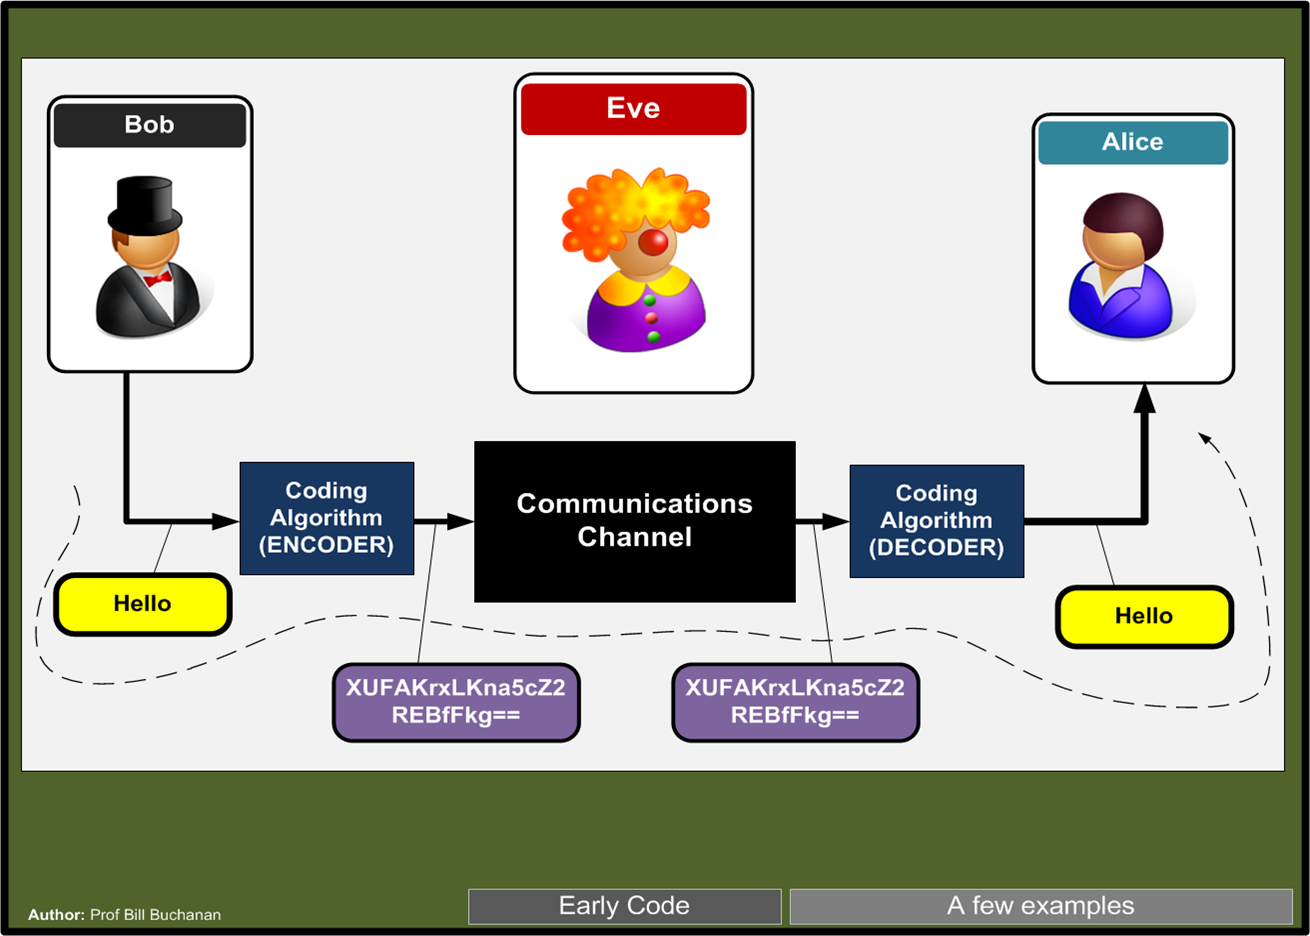
\includegraphics[scale=0.4]{immagini/eve1.png}
\end{figure}

\subsection{Principio di Kerkof (1800)}
 ``l'attaccante sa tutto tranne la chiave e il contenuto del messaggio.''\\
Questo principio vuole far notare che un cifrario è forte solo se non usa dati al di fuori della chiave per crittare il messaggio. Si predilige inoltre un cifrario aperto in modo che si possa analizzare e capire se e dove ci sono le debolezze

\subsection{Modalità di attacco}
Eva generalmente ha 4 modalità di attacco:\\
\begin{itemize}
\item Ciphertex only: eva ha solo il testo cifrato e prova a decifrarlo fino ad ottenere un testo sensato
\item Known plaintext: eva ha il plaintext e il suo testo cifrato
\item Choosen plaintext: eva sceglie che info cifrare in modo da cercare casi particolari
\item Choosen Ciphertex: eva può decifrare del testo inventato da lei in cerca di casi particolari
\end{itemize}
\subsection{Tipi di cifrari}
Prima del 1970 esistono 2 tipi di cifrari simmetrici e la steganografia, successivamente nascono i cifrari asimmetrici. Questi ultimi sono meno veloci rispetto a quelli simmetrici. Un metro di valutazione efficace per valutare un cifrario è la sua resistenza all'attacco di tipo forza bruta (provando tutte le combinazioni possibili quanto ci metto mediamente ad "indovinare" la chiave?). La soluzione possibile per risolvere questo attacco è di aumentare la chiave per multipli di 8 bit.

\section{cifrari storici}
\subsection{cifrari monoalfabetici a sostituzione}
\subsubsection{Cifrario di Cesare}
Si prende un valore x e si aggiunge un valore K il risultato, che indichiamo con y, è il testo cifrato:
\begin{center}
$y=(x+k)\mod26$
\end{center}
Vediamo ora come si può attaccare questo cifrario:\\
\textbf{Attacco Ciphertex only}: provo tutti i K fino a quando non riesco ad ottenere un plaintext sensato
\textbf{Attacco known plaintext}: sapendo che la lettera 't' è stata codificata con 'd' e sapendo che 't' è 19 e 'd' è 3 posso ottenere k:\\
$$(19+k)\mod26 = 3\mod26 \rightarrow k=10$$
\textbf{Attacco choosen plaintext}: dato che A è stato codificato con 1 cifro il testo 'A' e ottengo direttamente la chiave
\textbf{choosen Ciphertex}: provo a decrittare 'A' e ottengo -k
\subsubsection{Quadrato di polimio}
Si tratta di un quadrato $5 \times 5$

La scacchiera originale è costituita da una griglia composta da 25 caselle ordinate in cinque righe ed altrettante colonne. Le lettere dell'alfabeto vengono inserite da sinistra a destra e dall'alto in basso. Le righe e le colonne sono numerate: tali numeri sono gli indici o "coordinate" delle lettere costituenti il messaggio in chiaro:
\begin{center}
\begin{tabular}{c|c|c|c|c|c|}
 & 1& 	2& 	3& 	4& 	5\\
 \hline
 1& 	A& 	B& 	C& 	D& 	E\\
 2& 	F& 	G& 	H& 	I, J& 	K\\
3& 	L& 	M& 	N& 	O& 	P\\
4& 	Q& 	R& 	S& 	T& 	U\\
5& 	V& 	W& 	X& 	Y& 	Z\\
\end{tabular}
\end{center}



La trasposizione avviene sostituendo ad ogni lettera del messaggio un numero le cui cifre rappresentano il numero di riga e di colonna della sua posizione nella scacchiera. Ad esempio, operando sulla parola "WIKIPEDIA":\\

    la lettera "W" si trova nella 5ª riga e 2ª colonna, per cui il suo codice sarà 52;\\
    la lettera "I" si trova sulla 2ª riga e 4ª colonna, per cui il suo codice sarà 24;\\

Proseguendo con questo metodo il risultato finale per "WIKIPEDIA" sarà « 52 24 25 24 35 15 14 24 11 ».
\subsection{Cifrario affini}
Risulta molto simile a cesare solo che lo zero non si trova in 0 ma in q:

$$y=(mx+q)\mod26$$

Esempio: $y=9\cdot7+2\mod26 \leftarrow13$
Risulta quindi necesaria l'esistenza dell'\textbf{inverso moltiplicativo} in $Z_n$. Questa condizione è "gratis" se si lavora in un campo (con n numero primo) dove ho sempre l'inverso, se si lavora in un anello infatti non è detto che l'inverso esista sempre. Esiste una CNS se non si vuole usare un campo: se n e x sono coprimi (ovvero MCD(n,x)=1), dato che solitamente un campo $Z_n$ n è primo questa condizione è sempre verificata.
L'esempio precedente decifro y nel seguente modo:

$$x=\frac{1}{9}\cdot(y-2)\mod26$$
$$x=3\cdot(y-2)\mod26$$
$$x=7$$

l'inverso di $\frac{1}{9}$ lo si ottiene nel seguente modo:
$$9\cdot=1\mod26$$
$$x=3$$

\textbf{Attacco know plaintext} \\
Sappiamo che if(8,5)$\rightarrow$pq(15,16) allora:\\
$
\begin{cases}
15=8\cdot k+h \mod 26 \\
16 = 5\cdot k+h \mod26
\end{cases}
\rightarrow
\begin{cases}
k=17\\
h=9
\end{cases}
$
\newpage
\subsubsection{Problema analisi delle frequenze per i cifrari affini}
In questo tipo di cifrario si sfrutta la debolezza dell'alfabeto di riferimento (sappiamo che alcune lettere si ripetono con più frequenza se il plaintext è in italiano rispetto allo stesso plaintext di riferimento)
\begin{figure}[htbp]
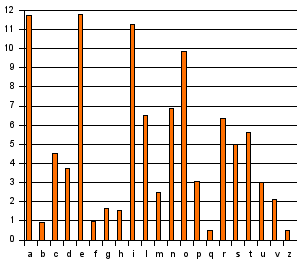
\includegraphics[scale=0.8]{immagini/Frequenze-alf_it.png}
\caption{frequenze delle lettere nell'alfabeto italiano}
\end{figure}

\subsection{Polialfabetici a sostituzione}
Risolvono il problema delle analisi delle frequenze facendo uso di un numero più o meno grande di alfabeti per sostituire le lettere del messaggio, usando un determinato ordine che costituisce la chiave. Esempio di cifrario polialfabetico è il cifrario di Vigenere. Si contrappone ai cifrari a sostituzione di tipo monoalfabetico quale ad esempio il cifrario di Cesare.

\subsubsection{Cifrario di Vigenere}
Il metodo si può considerare una generalizzazione del cifrario di Cesare; invece di spostare sempre dello stesso numero di posti la lettera da cifrare, questa viene spostata di un numero di posti variabile ma ripetuto, determinato in base ad una parola chiave, da concordarsi tra mittente e destinatario, e da scrivere ripetutamente sotto il messaggio, carattere per carattere; la chiave era detta anche verme, per il motivo che, essendo in genere molto più corta del messaggio, deve essere ripetuta molte volte sotto questo, come nel seguente esempio:\\
\begin{center}
\begin{tabular}{ll}
Testo chiaro &- RAPPORTOIMMEDIATO\\
Verme &- VERMEVERMEVERMEVE\\
Testo cifrato &- MEGBSMXFUQHIUUEOS\\
\end{tabular}
\end{center}
Il testo cifrato si ottiene spostando la lettera chiara di un numero fisso di caratteri, pari al numero ordinale della lettera corrispondente del verme. Di fatto si esegue una somma aritmetica tra l'ordinale del chiaro (A = 0, B = 1, C = 2...) e quello del verme; se si supera l'ultima lettera, la Z, si ricomincia dalla A.

\subsubsection{Debolezza del Cifrario di Vigenere: l'attacco di Kasinski}
Sfrutta l'attacco delle analisi delle frequenze dividendo il testo cifrato in n sottoistanze. Per far ciò si possono utilizzare metodi statistici per trovare n, e successivamente applicare l'analisi delle frequenze a ciascun alfabeto cifrante. Ovvero, se abbiamo come chiave VERME, basta operare l'analisi delle frequenze per tutte le lettere crittate dalla V, poi per quelle crittate dalla E, ecc. Perciò, la prima, la sesta, l'undicesima, ecc. lettera avranno lo stesso alfabeto cifrante. La parte più complicata sta dunque nello scoprire la lunghezza della chiave cifrante anche se la cosa non è impossibile. Nel testo cifrato infatti, se la chiave utilizzata è breve, vi saranno probabilmente delle serie di lettere ripetute. Queste serie di lettere, se abbastanza lunghe (5-6 caratteri), saranno generate probabilmente dalla stessa parola in chiaro. Basterà allora calcolare la distanza tra una parola e l'altra e la lunghezza della ripetizione per risalire alla lunghezza n della chiave. Così facendo si può capire quali lettere usano il primo alfabeto cifrante, quali il secondo, e così via procedendo poi con l'analisi delle frequenze per ciascun alfabeto.

\subsubsection{Cifrario di Gardano}
Risulta essere come Vigenere solo che la chiave è formata da chiave+plaintext. Ha come vantaggio una maggiore resistenza all'attacco di Kasinski

\subsubsection{Cifrario Playfair}
La tecnica cifra coppie di lettere (digrafi), invece che una singola lettera come nel semplice cifrario a sostituzione di Vigenère allora in uso. Playfair è quindi significativamente più difficile da forzare poiché l'analisi delle frequenze usata per i semplici cifrari a sostituzione non funzionano con esso. L'analisi delle frequenze può essere ancora intrapreso, ma sono possibili 600 digrafi [1] invece di 26 monografi. L'analisi della frequenza dei digrafi è possibile, ma considerevolmente più difficile. Inoltre le frequenze relative delle singole lettere hanno un intervallo molto più ampio di quello dei digrafi, rendendo l’analisi delle frequenze ulteriormente complicata. Per questi motivi, a suo tempo, il codice Playfair era considerato inviolabile.

\subsubsection{cifrario ADFGX}

Nella primavera del 1918 le truppe tedesche stavano pianificando una serie di attacchi in forze per sfondare le linee nemiche (Offensive di primavera) e dirigersi verso Parigi. Per rendere sicura la trasmissione dei piani di attacco alle truppe fu deciso di cifrare le comunicazioni mediante l'uso di un cifrario inventato dal colonnello Nebel denominato ADFGX, dalle uniche lettere che apparivano nel testo cifrato (in alcune versioni venivano usate le lettere ADFMX); tale cifrario derivava da un precedente schema crittografico noto come GEDEFU 18 (GEheimschrift DEr FUnker 18, o cifrario dei radiotelegrafisti 18). Le lettere del testo cifrato venivano selezionate da una scacchiera di dimensioni 5x5 (quindi con 25 possibili combinazioni) con l'unica differenza rispetto agli altri cifrari a trasposizione che per gli indici delle righe e delle colonne non erano usati numeri ma lettere (A, D, F, G e X, appunto). Essendo le possibili combinazioni solo 25, le 26 lettere dell'alfabeto non rientravano nello schema per cui fu scelto di cifrare le lettere "I" e "J" con lo stesso simbolo. La disposizione delle lettere nella scacchiera era data da una chiave che cambiava quotidianamente.

\subsection{cifrari a blocchi}
\subsubsection{cifrario di Hill (1929)}
È il primo cifrario che introduce l'algebra lineare e modulare.\\
Nella cifratura, ogni lettera è per prima cosa codificata in numero. Lo schema usato più di frequente è semplicemente: A = 0, B = 1, ..., Z = 25, ma questa non è una caratteristica essenziale del cifrario. Un blocco n di lettere è quindi considerato come uno spazio vettoriale di dimensione n, e moltiplicato per una matrice n x n, modulo 26 (se si usa un numero più alto di 26 nel modulo base, allora si può usare uno schema numerale diverso per codificare le lettere, ed è possibile anche utilizzare spazi e punteggiatura). L'intera matrice è considerata la chiave del cifrario e deve essere casuale, a patto che sia invertibile in $\mathbb{Z}_{26}^n$ (per assicurare che la decrittazione sia possibile). Considerando il messaggio 'TUO' e la seguente chiave (che in lettere sarebbe Y Y P R Z W I Z J):

    $$\begin{pmatrix} 24 & 24 & 15 \\ 17 & 25 & 22 \\ 08 & 25 & 09 \end{pmatrix} $$

Considerando che ‘T’ è ‘19’, ‘U’ è ‘20’ e ‘O’ è ‘14’, il messaggio è il vettore:

   $$ \begin{pmatrix} 19 \\ 20 \\ 14 \end{pmatrix}$$

Conseguentemente il vettore cifrato è dato da:

    $$\begin{pmatrix} 24 & 24 & 15 \\ 17 & 25 & 22 \\ 08 & 25 & 09 \end{pmatrix} \begin{pmatrix} 19 \\ 20 \\ 14 \end{pmatrix} = \begin{pmatrix} 1146 \\ 1131 \\ 778 \end{pmatrix} \pmod{26} \equiv \begin{pmatrix} 02 \\ 13 \\ 24 \end{pmatrix} $$

che corrisponde al testo crittato ‘CNY’.\\
Il calcolo è dato dalla moltiplicazione matrice $\times$ testo in chiaro. Dopo aver effettuato questo calcolo, al risultato si toglie il modulo (in questo caso 26) tante volte quante ne servono per avere come differenza un numero inferiore del modulo stesso e che dia, quindi, in risultato una lettera ben definita.

    $$C \leftarrow 02 = 24 \cdot 19 + 24 \cdot 20 + 15 \cdot 14 \pmod{26}$$
    $$N \leftarrow 13 = 17 \cdot 19 + 25 \cdot 20 + 22 \cdot 14 \pmod{26}$$
    $$Y \leftarrow 24 = 08 \cdot 19 + 25 \cdot 20 + 09 \cdot 14 \pmod{26}$$
    
Come si può notare la matematica dietro questo cifrario inizia a diventare complessa anche su esempi semplici.

\subsubsection{Proprietà dei cifrari a blocchi}
Nel 1950 Cloude Channon afferma che i codici devono avere 2 proprietà:
\begin{itemize}
\item Con una piccola modifica in input si deve generare una grossa variazione in output (proprietà di confusion)
\item Nel cipertext un singolo carattere deve dipendere da più carattere in input (proprietà di diffusion)
\end{itemize}
l'esempio principe di queste due proprietà è otp
\subsubsection{One Time Pad (OTP)}
In questo cifrario la chiave è una stringa pseudo casuale (quindi non predicibile) lunga quanto il plaintext che si usa per xorare bit a bit il plaintext rendendo quindi un cipertext unico. Questo è l'unico cifrario considerato sicuro ma il suo limite è come gestire la chiave dato che risulta essere lunga, difficile da spedire e generare. Esiste un metodo migliore? Si con le funzioni one way è facile arrivare nel codominio ma è difficile tornare nel dominio inziale.

Esempio:
$x_j=x^2_{j-1}\mod n$

Dove il risultato finale è formato dai bit meno significativi del risltato della potenza.
\subsubsection{linear feedback shift register (LFSR)} 
Gli LFSR possono essere implementati in hardware, e ciò li rende utili in applicazioni che richiedono la generazione molto rapida di numeri pseudo-casuali, come nella tecnica radio Direct Sequence Spread Spectrum, usata ad esempio nell'UMTS.

Il Global Positioning System (GPS) usa gli LFSR per trasmettere rapidamente una sequenza che indica degli istanti relativi ad alta precisione, sfruttandone il determinismo: basta infatti trasmettere il seme utilizzato nel trasmettitore e la sequenza generata sarà identica anche sul ricevitore.

\section{Problemi difficilmente risolubili}
Come vedremo prossimamente i cifrari moderni sono considerati sicuri non quanto per la complessità delle loro operazioni ma dalla difficoltà di fattorizzare (trovare i numeri primi il cui prodotto forma il numero) i numeri "grandi" in poco tempo. Vediamo ora alcuni teoremi a riguardo.

\subsection{Teorema dei numeri primi}
Se $\pi(x)$ è il numero di numeri primi minori di x allora:
$$\pi(x) \sim \frac{x}{\log x}$$
Ovvero che ci sono ``tanti'' numeri primi
\begin{itemize}
\item Ogni intero positivo è prodotto di numeri primi, questa fattorizazione è unica a meno dell'ordine dei fattori
\item Si usa l'algoritmo di euclide: il resto che precede lo 0 è il MCD(a,b)
\end{itemize}
Esempio:\\
$\text{MCD} (1180,482) \rightarrow
1180 = 2 \cdot 482+216 \rightarrow
482 = 2 \cdot 216+50 \rightarrow
216 = 4 \cdot 50+16 \rightarrow
50 = 3 \cdot 16+2 \rightarrow
16 = 8 \cdot 2 +0$\\
\textbf{Vantaggi}:
\begin{itemize}
\item Non richiede la fattorizzazione dei numeri primi
\item È veloce
\end{itemize}

\subsection{Proprietà delle congruenze}
Siano a,b due interi non nulli e sia d=mcd(a,b) allora esistono due interi x e y tc $ax+by=d$. In particolare se a e b sono primi tra loro allora esistono due interi x e y tc $ax+by=1$

\subsection{Algoritmo di Euclide esteso}
Precondizione:\\
Se MCD(a,n)=1 $\exists$ inverso
$a \cdot s+n \cdot t = 1 \mod n$\\
$a \cdot s \equiv 1 \mod n$

\subsection{Teorema cinese dei resti}
Si usa il teorema cinese dei resti per velocizare i conti in modulo. Serve per spezzare una congruenza $\mod (n)$ in un sistema di congruenze in $\mod(fattori di n)$.
\textbf{definizione}: siano m ed n due interi positivi tc $mdc(m,n)=1$ dati a,b interi $\exists$ soluzione x(con $\! \! \! \mod(m\cdot n)$) del sistema di congruenze:

$\begin{cases}
x \equiv a \mod(n) \\
x \equiv b \mod(m)
\end{cases}$

Esempio:\\
$
p= r_1 \cdot r_2 \cdot r_3 \cdot ... \cdot r_n \\
p_i=\frac{P}{r_i} \\
q_i=p_i^{-1} \mod r_i\\
x \equiv pippo \mod p \Rightarrow
\begin{cases}
x=a_1 \cdot \mod r_1 \\
x=a_2 \cdot \mod r_2 \\
x=a_3 \cdot \mod r_3 \\
. \\
. \\
. \\
x=a_n \cdot \mod r_n
\end{cases}
\Rightarrow x= \sum\limits_{i=1}^{n} a_i \cdot p_i \cdot q_i \mod p
$
\subsection{Teorema di fermat}
$a^{p-1} \equiv 1 \mod p$ Se p è primo e a qualsiasi \\
\textbf{teorema di eulero-fermat}\\
$a^{\phi(1)} \equiv 1 \mod p$ se MCD(a,n)=1 con a qualsiasi e n qualsiasi
\textbf{Funzione di Eulero}\\
Dato n:\\
\begin{itemize}
\item se è primo $\phi(n) = n-1$
\item se è composizione di due primi allora $p \cdot q \Rightarrow \phi(n)= (p-1)\cdot (q-1)$
\item se è composizione di più di due primi allora $\phi(n) = n \cdot \pi(1-\frac{1}{p}) $
\end{itemize}
\section{Cifrari a chiave asimmetrica}
\subsection{Prefazione}
Nati nel 1970 nascono i cifrari con chiave asimmetrica, che dove ci si ritrova per la prima volta con due chiavi: una pubblica che consegnero ad alice per cifrare il messaggio e una privata che la userò per decifrare il messaggio. Idealmente:
\begin{itemize}
\item Alice chiede a Bob di spedirle il suo lucchetto, già aperto. La chiave dello stesso verrà però gelosamente conservata da Bob.
\item Alice riceve il lucchetto e, con esso, chiude il pacco e lo spedisce a Bob.
\item Bob riceve il pacco e può aprirlo con la chiave di cui è l'unico proprietario.
\end{itemize}

\begin{figure}[htbp]
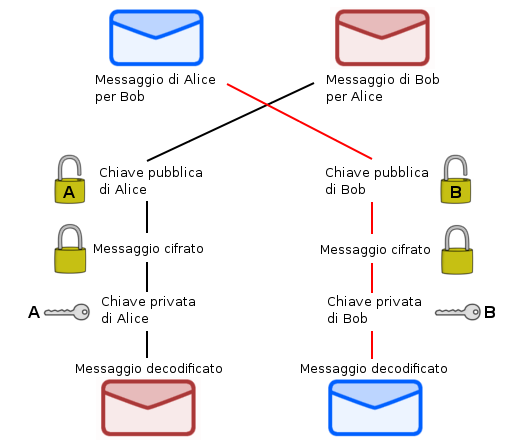
\includegraphics[scale=0.4]{immagini/Crittografia_asimmetrica_schema.png}
\end{figure}

Un'altro vantaggio di usare la crittografia asimetrica è la riduzione del numero di chiavi, vediamolo con un esempio:\\

Se 10 persone volessero comunicare in maniera simmetrica ho $\binom{10}{2} = 45$ chiavi. Nel caso assimetrico invece ho solo 20 chiavi. Le chiavi sono di meno nel caso di grandi numeri mentre con piccoli numeri risultano essere di meno quello simmetriche. Con i cifrari asimmetrici il ciphertext è computazionalmente intrattabile.
\subsection{RSA}
Il funzionamento di RSA è molto semplice: basta infatti eseguire una potenza in modulo. Vediamo ora i passi nel dettaglio
\subsubsection{Generazione della chiave}
La generazione delle due chiavi si divide in 5 parti:
\begin{itemize}
\item Scegli due primi $p$ e $q$ primi molto grandi (almeno 1024 bit) in maniera casuale
\item Calcola il valore n tc $n = p \cdot q$
\item Calcola $\phi(n) = \phi(p) \cdot \phi(q) = (p - 1)(q - 1) = n - (p + q -1)$ (dove $\phi$ è la funzione di eulero)
\item Scegli un valore $1<e<\phi(n)$ tc MCD$(e, \phi(n))=1 \Rightarrow$ MCD$(e,(p-1)\cdot(q-1))$
\item Calcola d tc $d \equiv e^{-1} \mod (\phi(n))$
\end{itemize}

Alla fine di questo procedimento abbiamo le due chiavi, quella pubblica è formata dalla coppia (n,e) mentre quella privata dalla terna (p,q,d)

\subsubsection{Come funziona RSA nella pratica}
Cifratura:\\
ciphertext = $plaintext^e \mod(n)$\\
Decifratura:\\
plaintext: $ciphertext^d \mod(n)$\\ \\
Esempio:\\
plaintext = 88, $K_pubblica(187,7), K_privata(p,q,d)$
ciphertext: $88^7 \mod(187) \Rightarrow 11$\\
plaintext: $11^23 \mod(187) \Rightarrow 88$\\
Bisogna fare attenzione che il messaggio deve essere al più uguale alla dimensione $n$ se il messaggio è di dimensione più grande si divide in ``parti'' che hanno dimensione $n$

\subsubsection{Dimostrazione corettezza RSA}

Siano $p,q$ primi tc $MCD(e,\phi(n))=1$ e:\\
$e\cdot d \equiv 1 \mod(\phi(n))$\\
$ciphertext: plaintext^e \mod(n)$\\
$plaintext: ciphertext^d \mod(n)$\\
Allora possiamo dire che:
$(ciphertext)^d \mod(n) \equiv ((plaintext)^e)^d \mod(n) \equiv plaintext^{e\cdot d} \mod(n)$\\
Vogliamo ora riscrivere $e \cdot d$ in una maniera più comoda, sfruttiamo quindi la funzione di Eulero tenendo a mente 3 cose:\\
\begin{itemize}
\item[1)]$\phi(n) = \phi(p\cdot q) = (p-1)\cdot(q-1)$
\item[2)]$e\cdot d = 1 \cdot \mod(\phi(n))$
\item[3)]$e\cdot d = 1 \cdot K\cdot \phi(n)$
\end{itemize}
Riscriviamo ora $e \cdot d$:\\
$(plaintext)^{K \cdot \phi(n)+1}\mod(n) = (plaintext)^{k\cdot(p-1)\cdot(q-1)+1}\mod(n)\equiv plaintext$\\
Dimostriamo ora che quanto scritto è corretto, semplifichiamo la dimostrazione e spezziamola in 3 parti: la prima parte dimostriamo per p la seconda parte per q ed infine per $p\cdot q$:\\
$(plaintext)^{k\cdot(p-1)\cdot(q-1)+1}\mod(n)=m$ sfrutto il teorema cinese dei resti:\\
$m\mod(q\cdot p) \Rightarrow \begin{cases}a\mod p \\b\mod q\end{cases}$

divido quindi l'ipotesi in due parti:
\begin{center}
$\begin{cases}
(m)^{k\cdot(p-1)\cdot(q-1)+1}\mod(p)\equiv m \mod(p) (1)\\
(m)^{k\cdot(p-1)\cdot(q-1)+1}\mod(q)\equiv m \mod(q) (2)
\end{cases}
$\\
\end{center}

Iniziamo a dimostrare la prima congruenza:\\
Ci sono due casi:
\begin{center}
$\begin{cases}
MCD(p,m)\not=1\\
MCD(p,m)=1
\end{cases}
$\\
\end{center}
Se siamo nel primo caso p e m non sono coprimi ma dato che p è primo allora sicuramente m è un multiplo di p quindi:\\
$m\equiv 0 \mod(p) \Rightarrow (m)^{k\cdot(p-1)\cdot(q-1)+1}\mod(p)\equiv m \mod(p)  \forall e,d$\\
Se invece siamo nel secondo caso allora:\\
$m^{(p-1)} \equiv 1 \mod(p) \Rightarrow [m^{(p-1)}]^{k\cdot (q-1)}\cdot m \mod(p) \equiv m $ Dato che 1 è l'elemento neutro della moltiplicazione (così come le sue potenze) $ \Rightarrow 1^{k\cdot (q-1)}\cdot m \mod(p) \equiv 1^{k\cdot(q-1)}\cdot m$

La seconda congruenza si risolve come la prima, e dato che anche q è primo

$$(m)^{K \cdot \phi(n)+1}\mod(n) \equiv m \mod(n) $$
$$(m)^{K \cdot \phi(n)+1} - m\mod(n) \equiv 0 \mod(n)$$
dato che il valore a sinistra è divisibile sia per q che per p $\Rightarrow \frac{(m)^{K \cdot \phi(n)+1} - m}{p\cdot q}$

\subsubsection{Attacchi ad RSA}

%ho due casi:\\
%\begin{center}
%$\begin{cases}
%MCD(p,m) \not= 1\\
%MCD(p,m) = 1
%\end{cases}
%$\\
%\end{center}

\end{document}

